\documentclass[dvipdfmx]{jsarticle}
\usepackage{tikz}
\usetikzlibrary{arrows}
\usetikzlibrary{intersections, calc}
\begin{document}
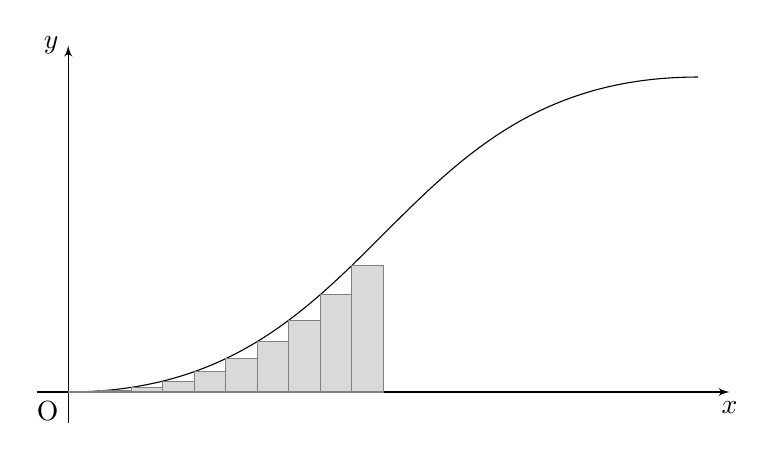
\begin{tikzpicture}[x=2cm,y=2cm,>=latex']

\def\width{0.2};

\node(O) at (0,0) [below left]{$\mathrm{O}$};
\draw[->] (-0.2,0) -- (4.2,0) node[below]{$x$};
\draw[->] (0,-0.2) -- (0,2.2) node[left]{$y$};

\draw[name path=graph] (0,0) .. controls (2,0) and (2,2) .. (4,2);

\foreach \x in {0,...,9} {
    \path[name path global/.expanded=path-\x](\width*\x,0) -- (\width*\x,2);
    \path[name intersections={of=graph and path-\x}];
    \coordinate (p-\x) at (intersection-1);
    \filldraw[fill=gray!30,draw=gray] ($(0,0)!(p-\x)!(1,0)$) rectangle ($(p-\x)+(\width,0)$);
}

\end{tikzpicture}
\end{document}